\documentclass[11pt]{article}

\usepackage{amsmath}
\usepackage{textcomp}
\usepackage[top=0.8in, bottom=0.8in, left=0.8in, right=0.8in]{geometry}
\usepackage{listings}
\usepackage{graphicx}
\usepackage{subcaption}


% Add other packages here %


% Put your group number and names in the author field %
\title{\bf Excercise 3\\ Implementing a deliberative Agent}
\author{Group 24: Benvenuti, Bronner}


% N.B.: The report should not be longer than 3 pages %


\begin{document}
\maketitle

\section{Model Description}
Here's how we modelised the problem.
\subsection{Intermediate States}
% Describe the state representation %
A State is defined by :
\begin{itemize}
	\item The city in  which the vehicle is currently in.
	\item The list of tasks currently carried by the vehicle.
	\item The list of tasks currently available for pickup.
\end{itemize}

\subsection{Goal State}
% Describe the goal state %
A goal state is reached when the vehicle isn't carrying any state and there are no task available for pickup.

\subsection{Actions}
% Describe the possible actions/transitions in your model %
An action consists of either going to a city to deliver a task or going to a city to pickup a task.

\section{Implementation}

\subsection{BFS}
% Details of the BFS implementation %
\paragraph{State class} The state class is defined in State.java and implement our representation of a state. It also contain the list of action performed to reach this state and the cost of the state.

The way the search work is the following: we start from the state we're currently in and compute all the possible actions and resulting states. Those new states are inserted at the bottom of a linked list. Once we've computed all the next states we poll the one on the top of the linked list and repeat.

Before computing the next state we check if the state is a goal state or if we have already visited this state once. Checking to see if the state is a goal state is pretty straightforward (we call the HashSet.isEmpty() function on the set of tasks carried by the vehicle and the set of task still available in the world). To see if we've already visited this state we insert every new state to a HashSet. When a new state is polled from the linked list, we can quickly (O(1)) check if it's already in the set.

Due to how we coded the State class our definition of a state in the BFS case differs from the definition we offered in section 1.1 because the hashing of two states where the vehicle is in the same city, carry the same tasks and where there are the same tasks still available for pickup will be different if the list of action performed or if the cost of the state is different. 

We could improve the efficiency of this method by not encoding the cost of the state in the state class. However this could result in a similar state but with a lower cost being dismissed by the algorithm if a less optimal path to the state was discovered before.
\subsection{A*}
% Details of the A* implementation %
The A* implementation is similar to the BFS with a few differences:

\begin{itemize}
	\item The new state are put in a priority queue instead of a linked list and the priority queue is sorted so that the next state to be pulled is the one expected by the heuristic to be optimal.
	\item To check if a state has been visited before, we first save his cost in a variable then set the state cost to zero and the list of of action performed to reach to state to null. We then enter the cost that we saved beforehand in a hashmap where the keys are the hash value of the states once their cost has been set to zero and their list of action performed has been set to null. This allows us to check if a state in the sense of our definition in section 1.1 has already been visited. If it's the case, we'll only pursue the new state if its cost is lower than the one that has already been visited.
\end{itemize}

\subsection{Heuristic Function}
% Details of the heuristic functions: main idea, optimality, admissibility %
The heuristic computes the distance from the city where the vehicle currently is to every city where there is currently a task to be picked up or where the vehicle can deliver one of the tasks he's currently carrying.

We tried two other heuristics, one where we would only look at the distance to the closest city where a package can either be delivered or picked up and another where we would compute the distance from the city where the vehicle currently is to every city where there is currently a task to be picked up or where the vehicle can deliver one of the tasks he's currently carrying and the distance between every city where the vehicle could pickup a package and the city where he had to deliver this package.

In all three cases those distances where multiplied by the cost per kilometer of the vehicle and added to the current state's cost. Out of the three the first one we presented resulted in the smaller number of iterations in the planning loop so we used it for the final version of our agent.
\section{Results}

\subsection{Experiment 1: BFS and A* Comparison}
% Compare the two algorithms in terms of: optimality, efficiency, limitations %
% Report the number of tasks for which you can build a plan in less than one minute %
We compare here the two algorithms BFS and A*. 

\subsubsection{Setting}
% Describe the settings of your experiment: topology, task configuration, etc. %
The two algorithms will be compared using the topology Switzerland, the politique of short distance. At first the number of tasks each algorithm is able to handle in less than one minute will be determinated (running on a I5 7600 with 16GB RAM).

Then the algorithms will be tested with different starting state to see if one consistently performs as least as well as the other and sometimes better. 10 tests with the highest possible number of tasks (5) will be performed. 
\subsubsection{Observations}
% Describe the experimental results and the conclusions you inferred from these results %
The limit of tasks for which a plan can be made in less than a minute is the following:
\begin{itemize}
  \item BFS: 5 tasks
  \item A*: 7 tasks
\end{itemize}
It should be noted that after this limit the computation fail on both algorithms. For the BFS an OutOfMemory occurs and a time out for the A*.

Both algorithms arrive each time at the same cost, which seems to indicate that both find the optimal solution. Moreover, for the 10 tests they have always outperformed the random algorithm. Therefore A* seems preferable to BFS as it will be able to be implemented for larger problems, for the same final result.

\subsection{Experiment 2: Multi-agent Experiments}
% Observations in multi-agent experiments %
The agents compute the plan with all the tasks that he can see, the task in the world and the tasks that they carry. Therefore, should another agent pick up a task, the whole plan must be recomputed.  
\subsubsection{Setting}
% Describe the settings of your experiment: topology, task configuration, etc. %
The topology is again Switzerland with 5 tasks. Now, the comparison will be made on the graph of the reward per km, see Figures \ref{img:multipleAgent}. There is now 1 to 3 agents in the world. 

\subsubsection{Observations}
% Describe the experimental results and the conclusions you inferred from these results %
Figures \ref{img:multipleAgent} show the result for 1, 2 or 3 agents in the world. This does not depend on the fact that the agent uses BFS or A*, only of the starting position (for a given starting state).
These Figures show the inefficiency to have more than one agent. Firstly, the mean reward per Km for respectively 2 and 3 agents is about 60\% and 50\% of the reward for only one agent. Secondly, some agent will move without being able to pick up a task because another would have been first. They will only stop when no more task will be available.
\begin{figure}
  \begin{subfigure}[b]{0.3\textwidth}
    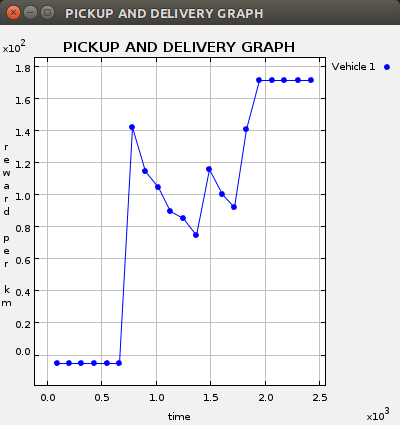
\includegraphics[width=\textwidth]{1agent.png}
    \caption{Single agent, BFS}
    \label{img:1agent}
  \end{subfigure}
  \begin{subfigure}[b]{0.3\textwidth}
    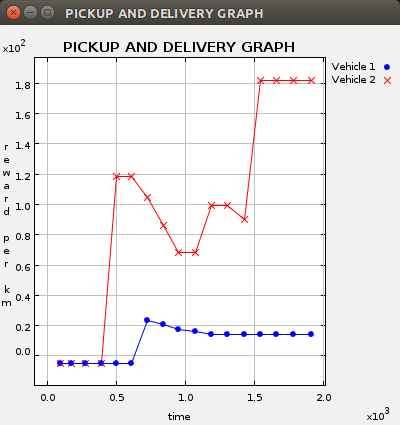
\includegraphics[width=\textwidth]{2agentsBFSASTAR.png}
    \caption{2 agents, BFS and A*}
    \label{img:2agents}
  \end{subfigure}
  \begin{subfigure}[b]{0.3\textwidth}
    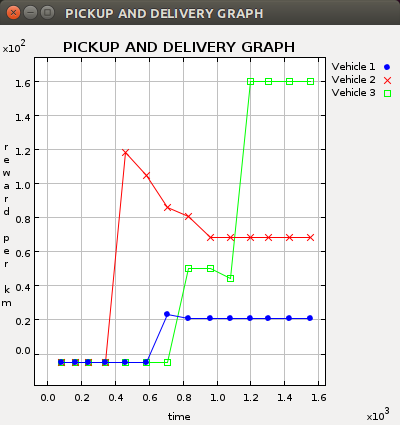
\includegraphics[width=\textwidth]{3agentsBBA.png}
    \caption{3 agents, BFS, BFS, A*}
    \label{img:3agents}
  \end{subfigure}
  \caption{Behavior of the agents depending on their number in the world.}
  \label{img:multipleAgent}
\end{figure}
\end{document}
